%% ----------------------------------------------------------------------------
%%  §8.5  Appendice: uniforme continuità, teorema di Cantor, funzioni lipschitziane
%% ----------------------------------------------------------------------------
\section{Appendice: uniforme continuità e funzioni lipschitziane}
\label{sec:uniforme-continuita}

Allo scopo di dimostrare che una funzione continua in un intervallo chiuso e limitato è
integrabile secondo Riemann, introduciamo in questo paragrafo il concetto di
\emph{uniforme continuità}. Vediamo prima perché la continuità, da sola, non basta al
nostro scopo. Per applicare il criterio di integrabilità occorre una partizione in cui
\emph{tutte} le oscillazioni $M_{k}-m_{k}$ siano piccole; se gli intervalli hanno
ampiezza minore di un certo $\delta$, ciò significa che $f$ deve variare poco su
\emph{ogni} intervallo di ampiezza $\delta$, ovunque esso si trovi. La continuità
garantisce qualcosa di più debole.

Sia $f$ continua in un intervallo $I$. Per la \cref{prop:caratt-continuita}, per ogni
$x_{0}\in I$ e per ogni $\epsilon>0$ esiste $\delta=\delta(x_{0},\epsilon)>0$ tale che
$\abs{f(x)-f(x_{0})}<\epsilon$ per ogni $x\in I$ con $\abs{x-x_{0}}<\delta$. Il numero
$\delta$ dipende, in generale, \emph{sia da $\epsilon$ sia da $x_{0}$}.

\begin{esempio}[La funzione $x^{2}$ su $\R$]\label{es:x2-non-uniforme}
Sia $f(x)=x^{2}$, $x\in\R$. Fissato $\epsilon>0$, supponiamo che esista $\delta>0$,
dipendente soltanto da $\epsilon$ e non da $x_{0}$, tale che
\begin{equation}\label{eq:x2-uniforme-ipotesi}
  \abs{x-x_{0}}<\delta \ \implica\ \abs{x^{2}-x_{0}^{2}}<\epsilon \qquad\perogni x_{0}\in\R .
\end{equation}
Posto $x=x_{0}+h$ con $h=\frac\delta2$, si avrebbe
$\abs{(x_{0}+h)^{2}-x_{0}^{2}}=\abs{2x_{0}h+h^{2}}<\epsilon$ per ogni $x_{0}\in\R$. Ma ciò è
assurdo, perché per $x_{0}>\frac\epsilon{2h}$ si ha $2x_{0}h+h^{2}>\epsilon$. Dunque il
$\delta$ della continuità di $x^{2}$ non può essere scelto indipendentemente dal punto.
Più precisamente, per $x_{0}\ge0$ il più grande $\delta$ ammissibile è quello per cui
$(x_{0}+\delta)^{2}-x_{0}^{2}=\epsilon$ (a destra di $x_{0}$ la funzione cresce più
rapidamente che a sinistra), cioè
\begin{equation}\label{eq:delta-x2}
  \delta_{\max}(x_{0},\epsilon)=\sqrt{x_{0}^{2}+\epsilon}-x_{0}
  =\frac{\epsilon}{\sqrt{x_{0}^{2}+\epsilon}+x_{0}} ,
\end{equation}
che tende a zero per $x_{0}\to+\infty$: dove il grafico è più ripido, occorre restare più
vicini a $x_{0}$ per non far variare $f$ più di $\epsilon$ (\cref{fig:uniforme}, a
sinistra).
\end{esempio}

\begin{figure}[htb]
\centering
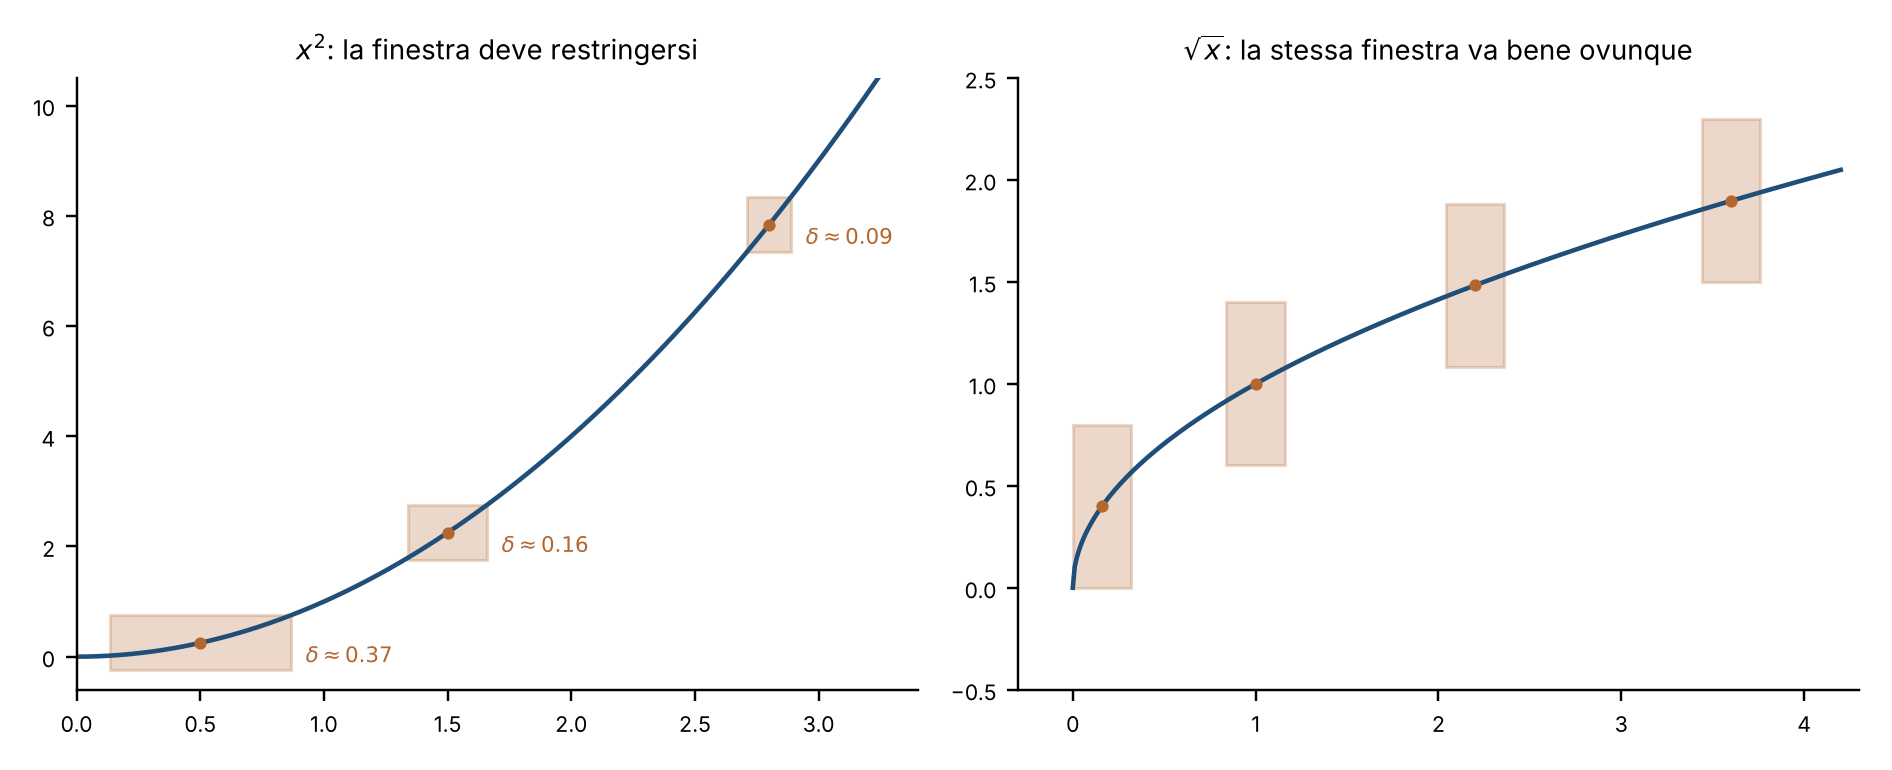
\includegraphics[width=\textwidth]{figure/uniforme.png}
\caption{A sinistra, $f(x)=x^{2}$ con $\epsilon=0{,}5$: per mantenere le variazioni di
$f$ entro $\pm\epsilon$, la finestra deve restringersi man mano che il grafico diventa
più ripido, e la sua semiampiezza è la \eqref{eq:delta-x2}. A destra,
$f(x)=\sqrt x$ con $\epsilon=0{,}4$: la stessa finestra, di semiampiezza
$\delta=\epsilon^{2}=0{,}16$, va bene ovunque, anche vicino all'origine dove la tangente è
verticale (\texttt{python/fig\_uniforme.py}).}
\label{fig:uniforme}
\end{figure}

È opportuno introdurre la definizione seguente.

\begin{definizione}[Funzione uniformemente continua]\label{def:uniformemente-continua}
\index{funzione!uniformemente continua}\index{uniforme continuità}
Si dice che $f:I\to\R$ è \emph{uniformemente continua} nell'intervallo $I$ se per ogni
$\epsilon>0$ esiste $\delta=\delta(\epsilon)>0$ tale che, per ogni $x,x'\in I$,
\begin{equation}\label{eq:uniforme-continuita}
  \abs{x-x'}<\delta \ \implica\ \abs{f(x)-f(x')}<\epsilon .
\end{equation}
\end{definizione}

La differenza con la continuità sta tutta nell'\emph{ordine dei quantificatori}.
Indicata con (C) la condizione
$\abs{x-x_{0}}<\delta\implica\abs{f(x)-f(x_{0})}<\epsilon$, si ha
\[
  \begin{aligned}
    &\text{continuità in } I: &&\perogni x_{0}\in I\ \ \perogni\epsilon>0\ \
    \esiste\delta>0\ \ \perogni x\in I : \ \text{(C)};\\
    &\text{uniforme continuità}: &&\perogni\epsilon>0\ \ \esiste\delta>0\ \
    \perogni x_{0}\in I\ \ \perogni x\in I : \ \text{(C)} .
  \end{aligned}
\]
Nella seconda riga $\delta$ viene scelto \emph{prima} del punto, e deve quindi andar bene
per tutti i punti. Una funzione uniformemente continua è ovviamente continua; il
viceversa è falso, come mostra l'\cref{es:x2-non-uniforme}. Geometricamente, $f$ è
uniformemente continua se un rettangolo di dimensioni fisse $2\delta\times2\epsilon$, fatto
scorrere con il centro sul grafico, è sempre attraversato dal grafico soltanto attraverso
i lati verticali (\cref{fig:uniforme}).

\begin{python}[Il $\delta$ massimo per $x^{2}$ e per $\sqrt x$]
import math

eps = 0.1
print("f(x) = x^2: delta massimo in x0, eps = 0.1")
for x0 in (0, 1, 10, 100, 1000):
    d = math.sqrt(x0**2 + eps) - x0            # formula (delta-x2)
    print(f"   x0 = {x0:7.2f}:  delta = {d:.3e}")
print("f(x) = sqrt(x): delta massimo in x0, eps = 0.1")
for x0 in (0, 0.0025, 1, 100, 1000):
    r = math.sqrt(x0)
    # a destra: (r + eps)^2 - x0;  a sinistra: x0 - (r - eps)^2
    d = 2 * eps * r + eps**2 if r < eps else 2 * eps * r - eps**2
    print(f"   x0 = {x0:7.4g}:  delta = {d:.3e}")
\end{python}
\begin{risultato}
f(x) = x^2: delta massimo in x0, eps = 0.1
   x0 =    0.00:  delta = 3.162e-01
   x0 =    1.00:  delta = 4.881e-02
   x0 =   10.00:  delta = 4.999e-03
   x0 =  100.00:  delta = 5.000e-04
   x0 = 1000.00:  delta = 5.000e-05
f(x) = sqrt(x): delta massimo in x0, eps = 0.1
   x0 =       0:  delta = 1.000e-02
   x0 =  0.0025:  delta = 2.000e-02
   x0 =       1:  delta = 1.900e-01
   x0 =     100:  delta = 1.990e+00
   x0 =    1000:  delta = 6.315e+00
\end{risultato}

Per $x^{2}$ il $\delta$ massimo decresce come $\frac\epsilon{2x_{0}}$; per $\sqrt x$, al
contrario, il più piccolo dei $\delta$ massimi è $\epsilon^{2}>0$ (lo si ha, ad esempio,
nell'origine):
come vedremo nell'\cref{es:radice-uniforme}, la radice quadrata è uniformemente continua
su tutta la semiretta $[0,+\infty)$.

\subsection{Il teorema di Cantor}

Riprendendo l'esempio di $x^{2}$: la funzione non è uniformemente continua su $\R$, ma lo
è in ogni intervallo chiuso e limitato $[a,b]$, grazie al teorema seguente.

\begin{teorema}[di Cantor]\label{teo:cantor}\index{teorema!di Cantor}
Sia $f$ una funzione continua nell'intervallo chiuso e limitato $[a,b]$. Allora $f$ è
uniformemente continua in $[a,b]$.
\end{teorema}

\begin{schema}
\Ipotesi{$f$ continua in $[a,b]$ (chiuso e limitato).}
\Tesi{$\perogni\epsilon>0\ \esiste\delta>0$ : $x,x'\in[a,b]$, $\abs{x-x'}<\delta\implica
\abs{f(x)-f(x')}<\epsilon$.}
\end{schema}

\begin{strategia}
Procediamo per assurdo. Se $f$ non è uniformemente continua, per un certo $\epsilon_{0}$
nessun $\delta$ funziona: scegliendo $\delta=\frac1n$ troviamo coppie di punti
$x_{n}$, $x_{n}'$ sempre più vicine, sulle quali però $f$ differisce di almeno
$\epsilon_{0}$. Qui entra in gioco l'ipotesi che l'intervallo sia chiuso e limitato:
per il teorema di Bolzano--Weierstrass i punti $x_{n}$ hanno un'estratta convergente a
un punto $x_{0}$ di $[a,b]$, e le $x_{n}'$ corrispondenti, vicinissime alle $x_{n}$,
convergono allo stesso punto. La continuità di $f$ in $x_{0}$ costringe allora
$f(x_{n})-f(x_{n}')$ a tendere a zero, in contraddizione con la scelta delle coppie.
\end{strategia}

\begin{dimostrazione}
Procediamo per assurdo. La definizione di uniforme continuità in $[a,b]$ si scrive
\[
  \perogni\epsilon>0\ \ \esiste\delta>0\ \ \perogni x,x'\in[a,b] : \
  \abs{x-x'}<\delta\implica\abs{f(x)-f(x')}<\epsilon ;
\]
la sua negazione afferma che esiste $\epsilon_{0}>0$ tale che, qualunque sia $\delta>0$,
esistono $x,x'\in[a,b]$ (dipendenti da $\delta$) con
\begin{equation}\label{eq:negazione-uc}
  \abs{x-x'}<\delta, \qquad \abs{f(x)-f(x')}\ge\epsilon_{0} .
\end{equation}
Scegliamo $\delta=\frac1n$, con $n\in\N$, e indichiamo con $x_{n}$, $x_{n}'$ i
corrispondenti punti di $[a,b]$ per cui vale la \eqref{eq:negazione-uc}:
\[
  \abs{x_{n}-x_{n}'}<\frac1n, \qquad \abs{f(x_{n})-f(x_{n}')}\ge\epsilon_{0}
  \qquad\perogni n\in\N .
\]
La successione $x_{n}$ è limitata, perché $a\le x_{n}\le b$; per il teorema di
Bolzano--Weierstrass (\cref{teo:bolzano-weierstrass}) esiste un'estratta $x_{n_{k}}$
convergente a un punto $x_{0}$; poiché $a\le x_{n_{k}}\le b$ per ogni $k$, per il
confronto dei limiti (\cref{cor:confronto-limiti}) anche $a\le x_{0}\le b$. È qui che
serve la \emph{chiusura} dell'intervallo. Inoltre
\[
  x_{n_{k}}-\frac1{n_{k}}<x_{n_{k}}'<x_{n_{k}}+\frac1{n_{k}} \qquad\perogni k\in\N,
\]
e poiché $n_{k}\ge k$ (\cref{lem:nk-maggiore-k}) si ha $\frac1{n_{k}}\to0$: per il teorema
dei carabinieri anche $x_{n_{k}}'\to x_{0}$. Le successioni $x_{n_{k}}$ e $x_{n_{k}}'$
sono formate da punti di $[a,b]$ e convergono a $x_{0}\in[a,b]$; per la continuità di
$f$ in $x_{0}$, nella forma (b) della \cref{prop:caratt-continuita},
\[
  \lim_{k\to+\infty}\bigl[f(x_{n_{k}})-f(x_{n_{k}}')\bigr]=f(x_{0})-f(x_{0})=0 ,
\]
in contrasto con il fatto che $\abs{f(x_{n_{k}})-f(x_{n_{k}}')}\ge\epsilon_{0}$ per ogni
$k$. La contraddizione prova la tesi.
\end{dimostrazione}

Entrambe le ipotesi sull'intervallo sono necessarie. Sulla semiretta $[0,+\infty)$,
che è chiusa ma non limitata, $x^{2}$ è continua ma non uniformemente continua
(\cref{es:x2-non-uniforme}); nell'intervallo $(0,1]$, che è limitato ma non chiuso, la
funzione $\frac1x$ è continua ma non uniformemente continua
(\cref{es:uno-su-x-non-uniforme}). In entrambi i casi la dimostrazione si inceppa nello
stesso punto: nel primo la successione $x_{n}$ può non essere limitata, e allora
un'estratta convergente può mancare; nel secondo l'estratta può convergere al punto
$0$, che non appartiene al dominio.

\subsection{Funzioni lipschitziane}

A conclusione del paragrafo riprendiamo una notevole classe di funzioni uniformemente
continue, già incontrata nel \cref{cap:applicazioni-derivate}.

\begin{definizione}[Funzione lipschitziana]\label{def:lipschitziana}
\index{funzione!lipschitziana}
Si dice che $f$ è \emph{lipschitziana} nell'intervallo $I$ se esiste una costante
$L\ge0$, detta \emph{costante di Lipschitz}, tale che
\begin{equation}\label{eq:lipschitziana}
  \abs{f(x)-f(x')}\le L\,\abs{x-x'} \qquad\perogni x,x'\in I .
\end{equation}
\end{definizione}

Per $x\neq x'$ la \eqref{eq:lipschitziana} afferma che le pendenze di tutte le
secanti al grafico sono comprese tra $-L$ e $L$: in ogni punto $(x',f(x'))$ il grafico è
contenuto nel «doppio cono» delimitato dalle rette di pendenza $\pm L$ passanti per quel
punto (\cref{fig:lipschitz}).

\begin{proposizione}[Le lipschitziane sono uniformemente continue]
\label{prop:lipschitz-uniforme}
Una funzione lipschitziana in un intervallo $I$ è uniformemente continua in $I$.
\end{proposizione}

\begin{schema}
\Ipotesi{$\abs{f(x)-f(x')}\le L\abs{x-x'}$ per ogni $x,x'\in I$.}
\Tesi{$f$ uniformemente continua in $I$.}
\end{schema}

\begin{strategia}
La \eqref{eq:lipschitziana} fornisce un $\delta$ esplicito, uguale per tutti i punti:
basta $\delta=\frac\epsilon L$.
\end{strategia}

\begin{dimostrazione}
Se $L=0$, $f$ è costante e la tesi è ovvia. Se $L>0$, fissato $\epsilon>0$ poniamo
$\delta=\frac\epsilon L$: per ogni coppia $x,x'\in I$ con $\abs{x-x'}<\delta$ si ha
$\abs{f(x)-f(x')}\le L\abs{x-x'}<L\delta=\epsilon$.
\end{dimostrazione}

Per le funzioni derivabili la lipschitzianità si legge sulla derivata.

\begin{teorema}[Funzioni derivabili e lipschitziane]\label{teo:lipschitz-derivata}
Sia $f$ derivabile nell'intervallo $I$. Allora $f$ è lipschitziana in $I$ con costante
$L$ se e solo se $\abs{f'(x)}\le L$ per ogni $x\in I$.
\end{teorema}

\begin{schema}
\Ipotesi{$f$ derivabile nell'intervallo $I$; \ $L\ge0$.}
\Tesi{$\abs{f(x)-f(x')}\le L\abs{x-x'}\ \perogni x,x'\in I \ \sse\ \abs{f'}\le L$ in $I$.}
\end{schema}

\begin{strategia}
Una implicazione è il corollario del teorema di Lagrange già dimostrato nel
\cref{cap:applicazioni-derivate}. Per l'altra, la \eqref{eq:lipschitziana} dice che i
rapporti incrementali sono in valore assoluto al più $L$, e il confronto dei limiti
trasmette la stima alla derivata.
\end{strategia}

\begin{dimostrazione}
Se $\abs{f'(x)}\le L$ per ogni $x\in I$, la \eqref{eq:lipschitziana} è la tesi del
\cref{cor:lipschitz}, conseguenza del teorema di Lagrange. Viceversa, sia $f$
lipschitziana con costante $L$ e sia $x\in I$. Per $h\neq0$ con $x+h\in I$ si ha
\[
  \biggl|\frac{f(x+h)-f(x)}h\biggr|\le L .
\]
Per $h\to0$ il rapporto incrementale tende a $f'(x)$, e il suo valore assoluto a
$\abs{f'(x)}$ (per la continuità del valore assoluto); per il confronto dei limiti
(\cref{teo:confronto-funzioni}(ii)) si ottiene $\abs{f'(x)}\le L$.
\end{dimostrazione}

\begin{esempio}[Tre funzioni a confronto]\label{es:lipschitz-esempi}
Tre esempi mostrano i legami tra derivabilità, lipschitzianità e uniforme continuità.
\begin{enumerate}[label=\textup{(\alph*)}]
  \item $\sen x$ è lipschitziana in $\R$ con costante $1$, perché
  $\abs{D\sen x}=\abs{\cos x}\le1$ per ogni $x$; la stessa disuguaglianza
  $\abs{\sen x-\sen x'}\le\abs{x-x'}$ era stata ottenuta nell'\cref{es:seno-lipschitz}
  con le formule di prostaferesi e la disuguaglianza $\abs{\sen t}\le\abs t$.
  \item $\abs x$ è lipschitziana in $\R$ con costante $1$, per la disuguaglianza
  triangolare inversa \eqref{eq:modulo-lipschitz}, ma non è derivabile in $0$: il
  \cref{teo:lipschitz-derivata} non si applica, e una funzione lipschitziana non è
  necessariamente derivabile.
  \item $\sqrt x$ è uniformemente continua in $[0,1]$ per il teorema di Cantor, ma non è
  lipschitziana: la pendenza della secante tra $0$ e $x$ è
  $\frac{\sqrt x-0}{x-0}=\frac1{\sqrt x}$, che tende a $+\infty$ per $x\to0^{+}$, mentre
  dovrebbe essere al più $L$. Equivalentemente, per il \cref{teo:lipschitz-derivata}
  applicato in $(0,1]$, la derivata $\frac1{2\sqrt x}$ non è limitata.
\end{enumerate}
\end{esempio}

\begin{figure}[htb]
\centering
\begin{tikzpicture}
\begin{axis}[name=l1, width=0.55\textwidth, height=4.6cm, axis lines=middle, axis on top,
  xmin=-0.3, xmax=6.5, ymin=-1.9, ymax=2.4, xtick=\empty, ytick=\empty,
  title={\scriptsize $\sen x$: il doppio cono di pendenza $\pm1$}]
  \fill[verde!15] (axis cs:2,0.909) -- (axis cs:6.3,5.209) -- (axis cs:6.3,-3.391)
    -- cycle;
  \fill[verde!15] (axis cs:2,0.909) -- (axis cs:-0.3,3.209) -- (axis cs:-0.3,-1.391)
    -- cycle;
  \addplot[verde!60!black, domain=-0.3:6.3] {0.909+(x-2)};
  \addplot[verde!60!black, domain=-0.3:6.3] {0.909-(x-2)};
  \addplot[curva, domain=-0.3:6.3, samples=120] {sin(deg(x))};
  \addplot[only marks, mark=*, mark size=1.6pt, rame] coordinates {(2,0.909)};
\end{axis}
\begin{axis}[at={(l1.east)}, anchor=west, xshift=0.7cm, width=0.5\textwidth,
  height=4.6cm, axis lines=middle, xmin=-0.05, xmax=1.1, ymin=-0.05, ymax=1.15,
  xtick=\empty, ytick=\empty, title={\scriptsize $\sqrt x$: secanti sempre più ripide}]
  \addplot[curva, domain=0:1.05, samples=200] {sqrt(x)};
  \addplot[rame, domain=0:1.05] {x};
  \addplot[rame, domain=0:0.3] {2*x};
  \addplot[rame, domain=0:0.12] {5*x};
  \addplot[rame, domain=0:0.055] {12*x};
  \addplot[only marks, mark=*, mark size=1.2pt, rame] coordinates
    {(1,1) (0.25,0.5) (0.04,0.2) (0.00694,0.0833)};
  \node[font=\scriptsize, rame, anchor=west] at (axis cs:0.9,0.82) {$1$};
  \node[font=\scriptsize, rame, anchor=west] at (axis cs:0.28,0.62) {$2$};
  \node[font=\scriptsize, rame, anchor=west] at (axis cs:0.11,0.62) {$5$};
  \node[font=\scriptsize, rame, anchor=south] at (axis cs:0.052,0.66) {$12$};
\end{axis}
\end{tikzpicture}
\caption{A sinistra, una funzione lipschitziana con costante $L=1$: il grafico di
$\sen x$ resta nel doppio cono verde, delimitato dalle rette di pendenza $\pm1$ per il
punto evidenziato, e così per ogni altro punto. A destra, le secanti al grafico di
$\sqrt x$ uscenti dall'origine hanno pendenze $1$, $2$, $5$, $12$, \dots, non limitate:
nessun cono di apertura finita contiene il grafico vicino all'origine.}
\label{fig:lipschitz}
\end{figure}

\begin{esempio}[La radice quadrata è uniformemente continua su $\lbrack0,+\infty)$]
\label{es:radice-uniforme}
Il teorema di Cantor non si applica alla semiretta, ma per la radice quadrata vale una
stima diretta: per $0\le x'\le x$,
\begin{equation}\label{eq:radice-holder}
  \sqrt x-\sqrt{x'}\le\sqrt{x-x'} .
\end{equation}
Infatti, elevando al quadrato i due membri non negativi di
$\sqrt x\le\sqrt{x-x'}+\sqrt{x'}$, la disuguaglianza equivale a
$x\le(x-x')+2\sqrt{x'(x-x')}+x'$, cioè a $0\le2\sqrt{x'(x-x')}$, che è vera. Dunque
$\abs{\sqrt x-\sqrt{x'}}\le\sqrt{\abs{x-x'}}$ per ogni $x,x'\ge0$, e posto
$\delta=\epsilon^{2}$ si ha $\abs{\sqrt x-\sqrt{x'}}<\epsilon$ non appena
$\abs{x-x'}<\delta$: la radice è uniformemente continua in $[0,+\infty)$ pur non essendo
lipschitziana. Una stima del tipo $\abs{f(x)-f(x')}\le L\abs{x-x'}^{\alpha}$, con
$0<\alpha\le1$, si chiama \emph{condizione di Hölder}; per $\alpha=1$ è la
lipschitzianità.
\end{esempio}

\begin{python}[Pendenze delle secanti: seno e radice quadrata]
import math, random

random.seed(1)
pend = []
for _ in range(100000):
    x, y = random.uniform(-10, 10), random.uniform(-10, 10)
    if x != y:
        pend.append(abs(math.sin(x) - math.sin(y)) / abs(x - y))
print(f"sen x: pendenza massima delle secanti = {max(pend):.6f}")
for h in (1e-2, 1e-4, 1e-6, 1e-8):
    print(f"sqrt(x): pendenza della secante tra 0 e {h:.0e}"
          f" = {math.sqrt(h) / h:7.0f}")
\end{python}
\begin{risultato}
sen x: pendenza massima delle secanti = 0.999970
sqrt(x): pendenza della secante tra 0 e 1e-02 =      10
sqrt(x): pendenza della secante tra 0 e 1e-04 =     100
sqrt(x): pendenza della secante tra 0 e 1e-06 =    1000
sqrt(x): pendenza della secante tra 0 e 1e-08 =   10000
\end{risultato}

Riassumendo, per una funzione definita in un intervallo valgono le implicazioni
illustrate nella \cref{fig:gerarchia}, nessuna delle quali si può invertire.

\begin{figure}[htb]
\centering
\begin{tikzpicture}[box/.style={draw=blu, fill=blu!8, rounded corners=2pt,
  font=\scriptsize, align=center, inner sep=4pt, minimum height=1.0cm,
  text width=1.95cm}]
  \node[box] (a) at (0,0) {derivabile con\\ $f'$ limitata};
  \node[box] (b) at (2.85,0) {lipschitziana};
  \node[box] (c) at (5.7,0) {uniformemente\\ continua};
  \node[box] (d) at (8.55,0) {continua};
  \draw[-Latex, thick, grigio] (a) -- (b);
  \draw[-Latex, thick, grigio] (b) -- (c);
  \draw[-Latex, thick, grigio] (c) -- (d);
  \node[font=\scriptsize, rame, align=center] at (1.425,-1.0) {$\abs x$ su $\R$};
  \node[font=\scriptsize, rame, align=center] at (4.275,-1.0) {$\sqrt x$ su $[0,1]$};
  \node[font=\scriptsize, rame, align=center] at (7.125,-1.05)
    {$x^{2}$ su $\R$,\\ $\frac1x$ su $(0,1]$};
\end{tikzpicture}
\caption{Le implicazioni tra le classi di funzioni in un intervallo. Sotto ciascuna
freccia, una funzione che appartiene alla classe di destra ma non a quella di sinistra.
Per un intervallo chiuso e limitato, il teorema di Cantor rende equivalenti le ultime
due classi.}
\label{fig:gerarchia}
\end{figure}

\begin{notastorica}[Dirichlet, Heine, Cantor]
Nella dimostrazione dell'integrabilità delle funzioni continue data da Cauchy nel 1823
c'era una lacuna: Cauchy usava senza accorgersene la continuità \emph{uniforme}, non
distinguendola da quella puntuale. La distinzione maturò negli anni successivi.
Peter Gustav Lejeune Dirichlet dimostrò il teorema che abbiamo chiamato di Cantor nelle
sue lezioni berlinesi del 1854 sugli integrali definiti, pubblicate però soltanto nel
1904. Il primo a pubblicare questi risultati fu Eduard Heine: la definizione di
uniforme continuità nel 1870, il teorema nel 1872, in un articolo sui fondamenti della
teoria delle funzioni nel quale riconosceva il proprio debito verso le idee di
Weierstrass e di Georg Cantor; per questo il teorema è noto anche come teorema di
Heine--Cantor. Rudolf Lipschitz considerò per la prima volta una condizione del tipo
\eqref{eq:lipschitziana} nel 1864, studiando la convergenza delle serie di Fourier; nel
1876 la pose come ipotesi che garantisce l'esistenza e l'unicità delle soluzioni delle
equazioni differenziali. È ancora oggi l'ipotesi standard dei teoremi di esistenza e
unicità che si incontrano, ad esempio, nello studio della dinamica del volo.
\end{notastorica}
